\documentclass{beamer}
\usepackage{sansmathaccent}
\pdfmapfile{+sansmathaccent.map}
\usepackage{comment}
\usepackage{physics}
\usetheme{Madrid}

\usepackage[utf8]{inputenc}
\usepackage{graphicx}

\title[21 cm]{Determining Galactic Strucutre through 21cm Emission Lines}
\author{Henry Shackleton}

\begin{document}

\titlepage

\section{Introduction and Theory}

\begin{frame}
  \frametitle{Hyperfine Strucutre of Hydrogen Emits 21cm Wavelenth Emission}
  \begin{columns}
    \begin{column}{0.7\textwidth}
      \begin{center}
  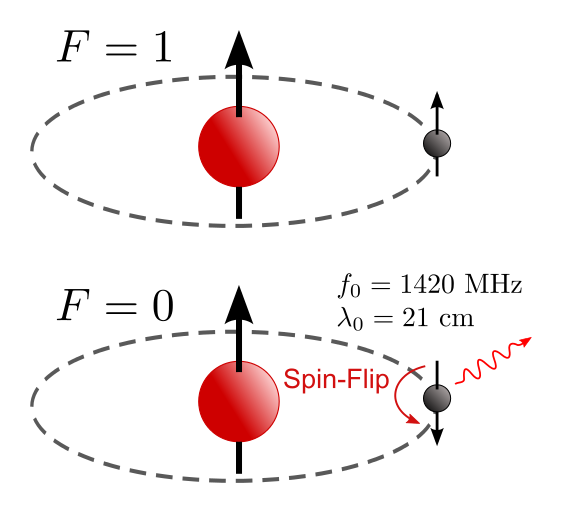
\includegraphics[width=0.7\linewidth]{hyperfine}
\end{center}
\end{column}
\begin{column}{0.3\textwidth}
  \begin{center}
    \begin{itemize}
      \item Hydrogen electron spin-flip causes electromagnetic radiation at a frequency of $1420.41$ MHz.
      \item Low probability ($2.9 \times 10^{-15} s^{-1}$), but the vast amount of hydrogen in the galaxy allows for this detection
    \end{itemize}\end{center}\end{column}\end{columns}
\end{frame}

\begin{frame}
  \frametitle{Doppler Shift Gives Change in 21cm Line Proportional to Velocity}
  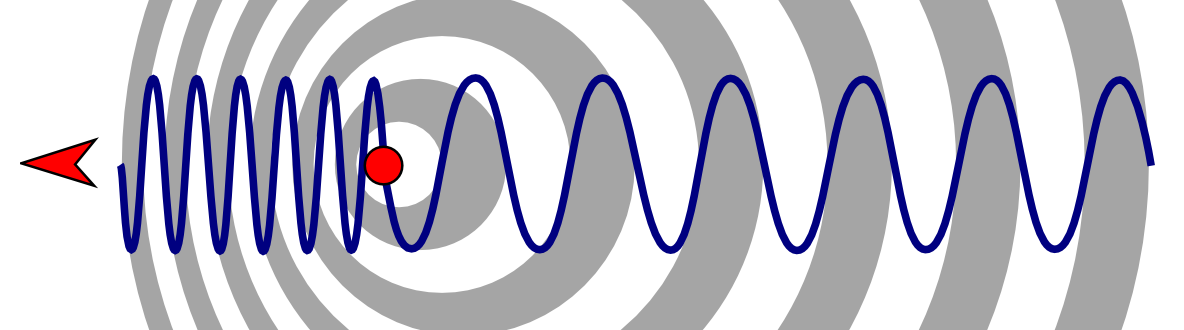
\includegraphics[width=1\textwidth]{diagrammatic}
  \begin{equation*}
  v = c \frac{1420.41 - \nu}{\nu}
\end{equation*}
\end{frame}

\begin{frame}
  \frametitle{Doppler Shift Gives Change in 21cm Line Proportional to Velocity}
  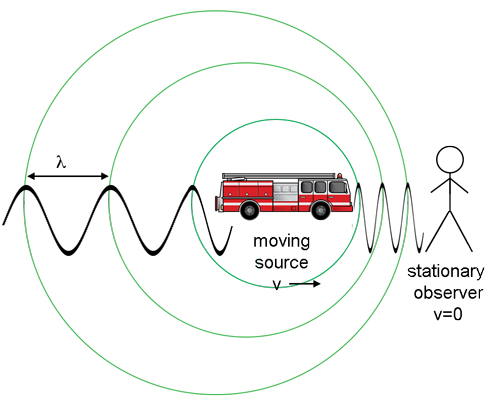
\includegraphics[width=0.75\textwidth]{siren_moving}
\end{frame}

\end{document}
